% textidote: ignore begin
\section{Application Domain Analysis}\label{sec:application-domain-analysis}
% textidote: ignore end

The following chapter provides an application domain analysis of the project.
The aim of such an analysis is to answer the question:
\textcquote[117]{mathiassen2018}{How will the target system be used?}
The analysis will be based on the actors and use cases of the system.
Section~\ref{subsec:actors} will introduce the \textit{Actors'} analysis that gives an overview of the different actors
interacting with the system and what their role is.
Section~\ref{subsec:use-cases} will introduce the \textit{Use Cases} analysis that describes the pattern of interaction
between the system and the actors in the application domain~\cite{mathiassen2018}.

\subsection{Actors}\label{subsec:actors}

An actor is a person, system, or external entity that interacts with the system~\cite{mathiassen2018}.
In this section, we will identify the actors that interact with the system and describe their roles and goals.
The relevant actors are the owner as seen in Table~\ref{tab:actor-owner}, the barista as seen in
Table~\ref{tab:actor-barista} and Cognito as seen in Table~\ref{tab:actor-cognito}.

\begin{table}[H]
    \noindent
    \rule{\textwidth}{0.4pt}

    \begin{center}
    \noindent
    \textit{\textbf{Owner Actor}}
    \end{center}

    \noindent
    \rule{\textwidth}{0.4pt}
    \noindent

    \textbf{Goal:} The owners interact with the system to gain insights into the performance of their assets
    and to make informed decisions based on the data provided.
    \newline
    \noindent

    \textbf{Characteristics:} The owners are the primary users of the system.
    They are experienced in managing day-to-day operations of the café, but they may not have extensive technical
    expertise.
    \newline
    \noindent

    \textbf{Examples:} One of the owners logs into the system on wednesday morning to prepare for the upcoming days.
    Their goal is to ensure that the café is well-staffed and that they have stocked up the right amount of baked goods
    for what they think will be a busy few days.
    Using the system, they can

    \begin{itemize}
        \item Check hourly sales data from the previous week to predict how many customers will
        visit the café.
        \item Optimize the schedule of the employees based on the predicted number of customers.
        \item Analyze the product demand to ensure that they have enough baked goods in stock.
    \end{itemize}

    \noindent
    \rule{\textwidth}{0.4pt}
    \caption{Actor specifications of the owner actor.
    }\label{tab:actor-owner}
\end{table}

\begin{table}[H]
    \noindent
    \rule{\textwidth}{0.4pt}

    \begin{center}
    \noindent
    \textit{\textbf{Barista Actor}}
    \end{center}

    \noindent
    \rule{\textwidth}{0.4pt}
    \noindent

    \textbf{Goal:} The baristas interact with the system to get an overview of the sales data and also to upload
    new data to the system.
    \newline
    \noindent

    \textbf{Characteristics:} The baristas are the employees that work in the café.
    They are responsible for serving the customers and keeping the café clean.
    The baristas are not expected to have any technical expertise.
    \newline
    \noindent

    \textbf{Example 1:} A barista logs into the system by typing in their credentials.
    When done typing in their credentials, they are presented with the sales data on the dashboard.
    They can see the sales data throughout the weeks and months.
    \newline
    \noindent

    \textbf{Example 2:} A barista logs into the system by typing in their credentials.
    They are looking to upload new sales data to the system.
    They navigate to the upload button and select the file they want to upload.

    \noindent
    \rule{\textwidth}{0.04pt}
    \caption{Actor specifications of the barista actor.
    }\label{tab:actor-barista}
\end{table}

\begin{table}[H]
    \noindent
    \rule{\textwidth}{0.4pt}

    \begin{center}
        \noindent
        \textit{\textbf{Cognito Actor}}
    \end{center}

    \noindent
    \rule{\textwidth}{0.4pt}
    \noindent

    \textbf{Goal:} The cognito actor interacts with the system to authenticate the users.
    \newline
    \noindent

    \textbf{Characteristics:} Cognito is a third-party service that provides authentication and authorization services.
    The cognito actor is not a person but a system that interacts with other systems to authenticate the users.
    \newline
    \noindent

    \textbf{Example 1:} When a user logs into the system using their username and password, the cognito actor
    authenticates the user and provides the system with the user's identity.
    \newline
    \noindent

    \textbf{Example 2:} When a user provides the system with an invalid username or password, the cognito actor
    denies the user access to the system and gives them an error message.

    \noindent
    \rule{\textwidth}{0.4pt}
    \caption{Actor specifications of the cognito actor.
    }\label{tab:actor-cognito}
\end{table}

\subsection{Use Cases}\label{subsec:use-cases}

In this section is an analysis of the use cases for the different actions actors can make in the solution.
This is done to get a better understanding of how the solution will apply to the problem.

\begin{table}[H]
    \begin{tabularx}{\textwidth}{ l X X X }
        \toprule
        \textbf{Use Case}
        & \textbf{Owner}
        & \textbf{Barista}
        & \textbf{Cognito}
        \\ \midrule
        Login
        & {\checkmark}
        & {\checkmark}
        & {\checkmark}
        \\ \midrule
        File uploading
        & {\checkmark}
        & {\checkmark}
        &
        \\ \midrule
        Diagram viewing
        & {\checkmark}
        & {\checkmark}
        &
        \\ \midrule
        Account handling
        & {\checkmark}
        &
        & {\checkmark}
        \\ \bottomrule
    \end{tabularx}
    \caption{Use cases for Owner, Barista, and Cognito.
    }\label{tab:actors-tabel}
\end{table}

% textidote: ignore begin
\subsubsection{Login}\label{subsubsec:login_usecase}
% textidote: ignore end

Login is an active action from a barista or an owner, where they provide a username or an e-mail and a password.
This action is then handled by Cognito, which verifies the credentials and responds with an error or a temporary token.
The token is then used as a prerequisite for other actions.
The Login action can be visualized through Figure~\ref{fig:cognito-conditional}

\begin{figure}[H]
    \centering
    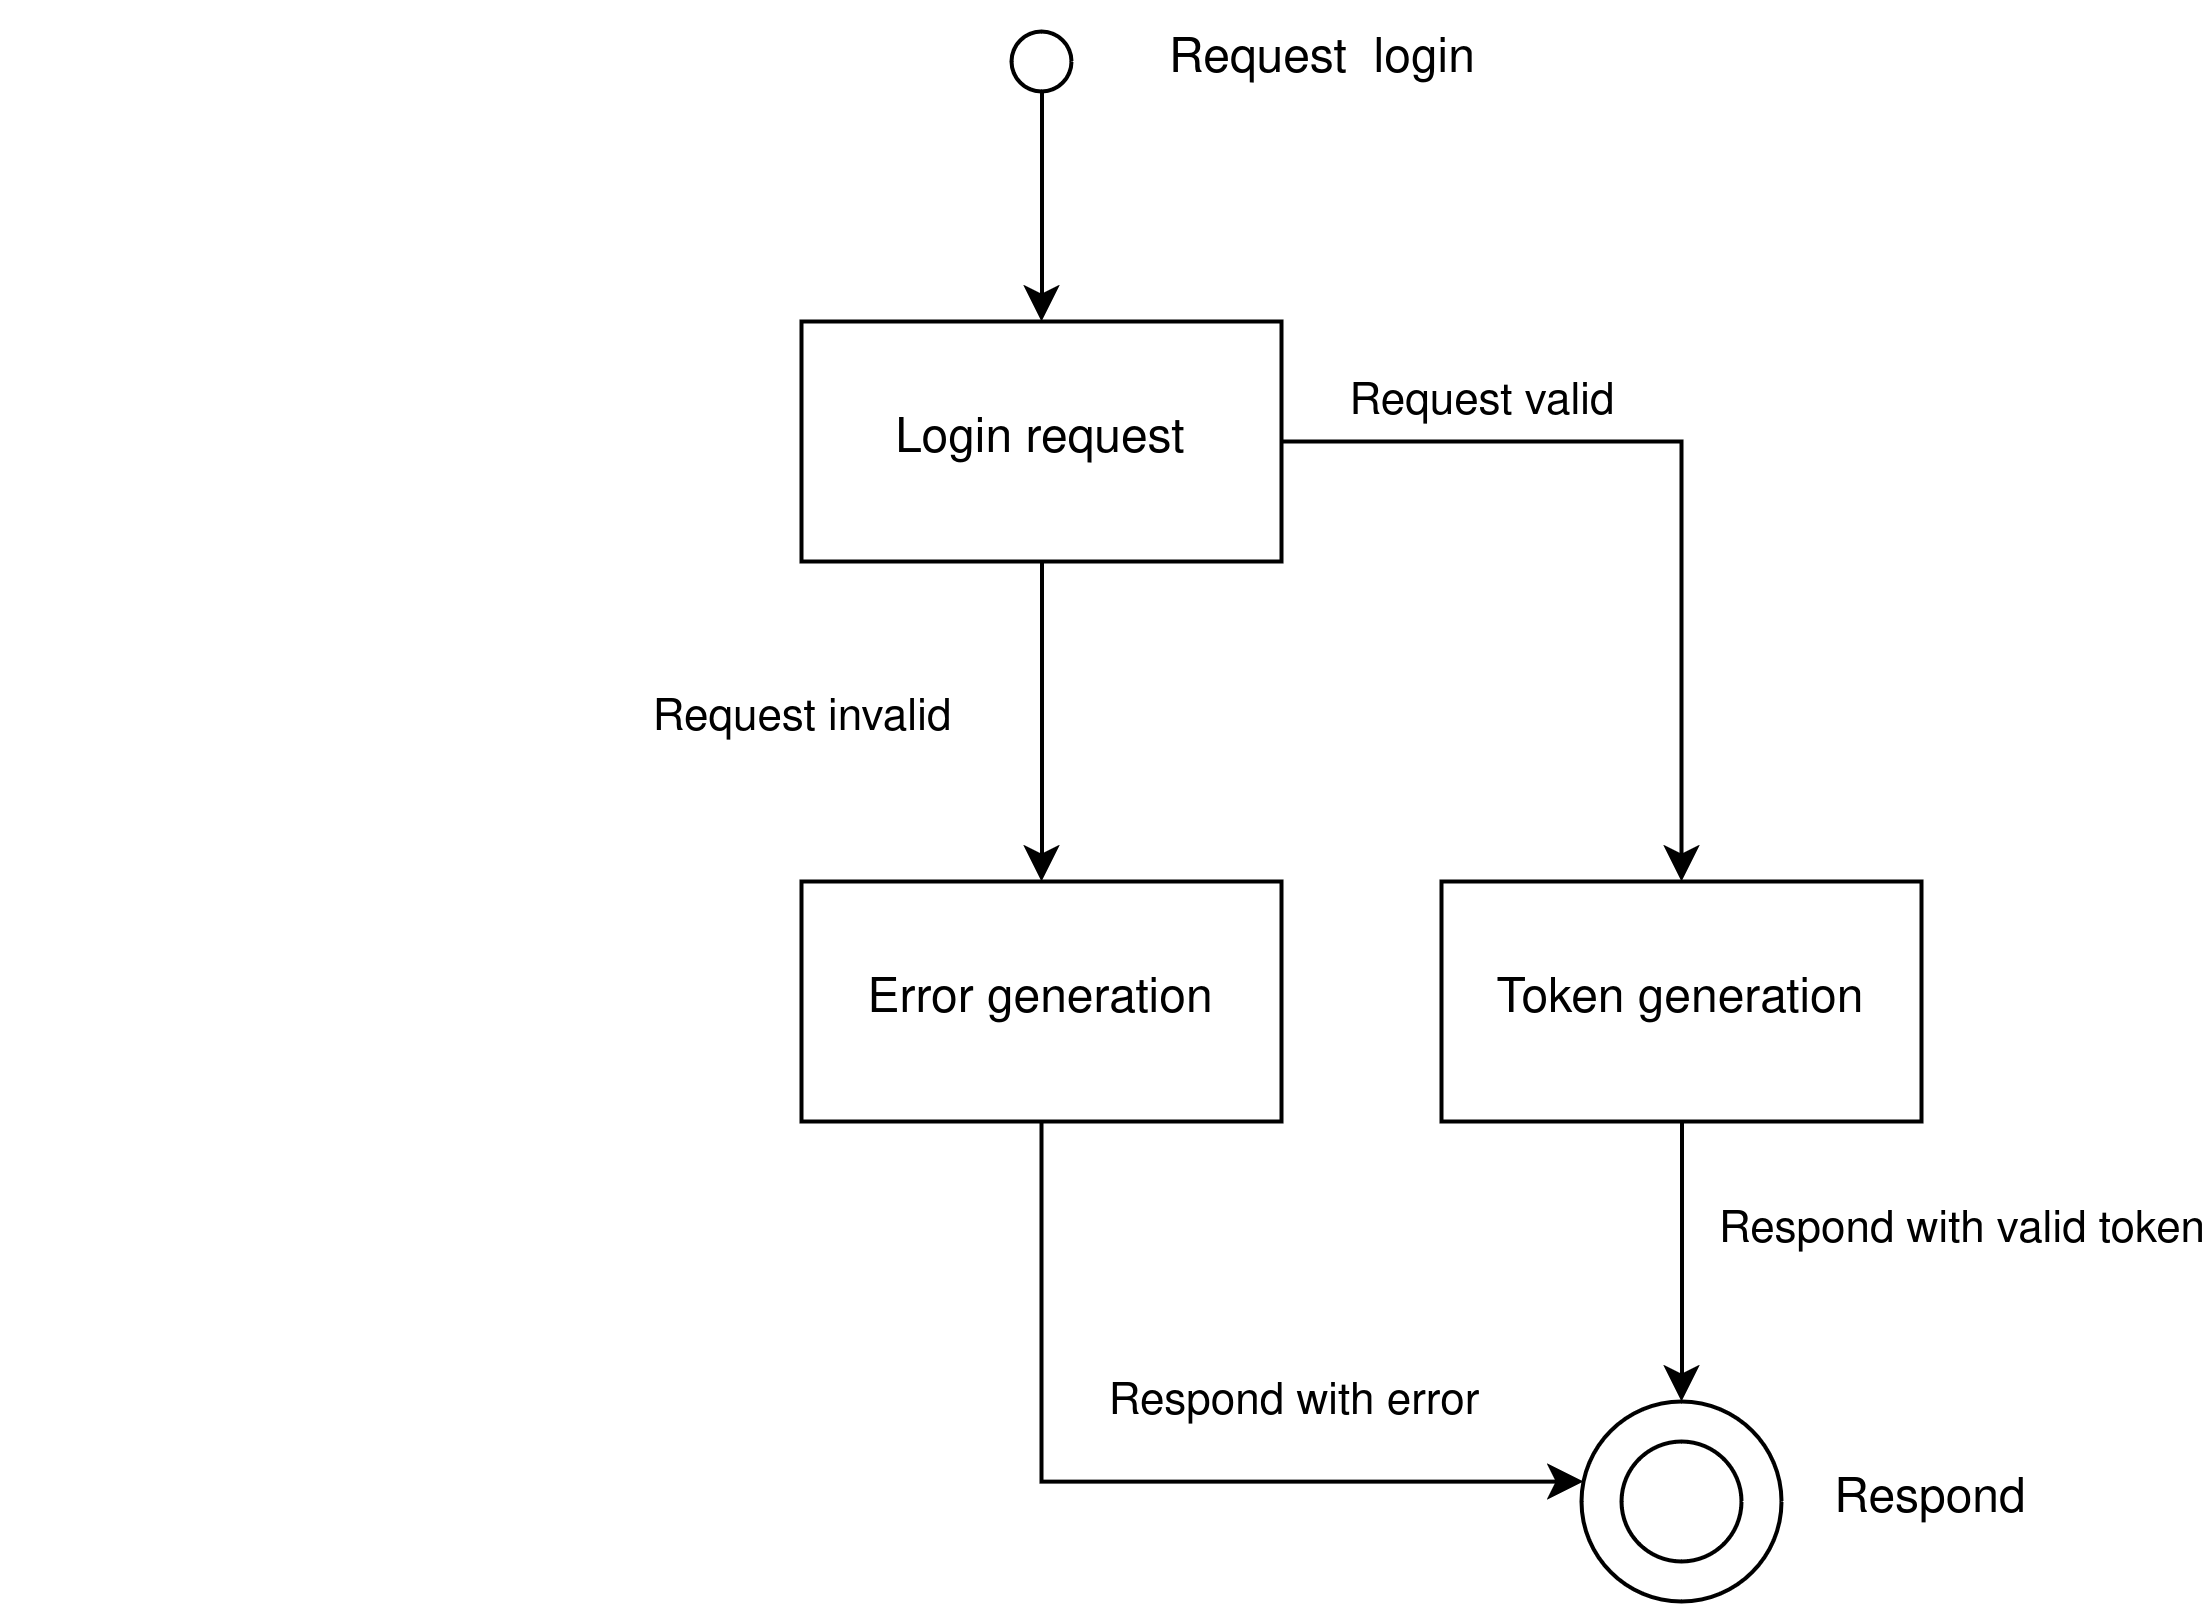
\includegraphics[width=0.75\textwidth]{ada-cognito}
    \caption{A diagram showing the Cognito actors use.
    }\label{fig:cognito-conditional}
\end{figure}

% textidote: ignore begin
\subsubsection{File uploading}\label{subsubsec:file_uploading_usecase}
% textidote: ignore end

Uploading a file is an action actively made by either an owner or a barista.
The action will be triggered by clicking on an upload button on the webpage and selecting the appropriate file.
The server will then validate and parse the file which will result in a success or error,
which will be shown to the user.
The workflow of uploading a file is shown in both Figure~\ref{fig:barista-conditional},
and Figure~\ref{fig:owner-conditional}.

\begin{figure}[H]
    \centering
    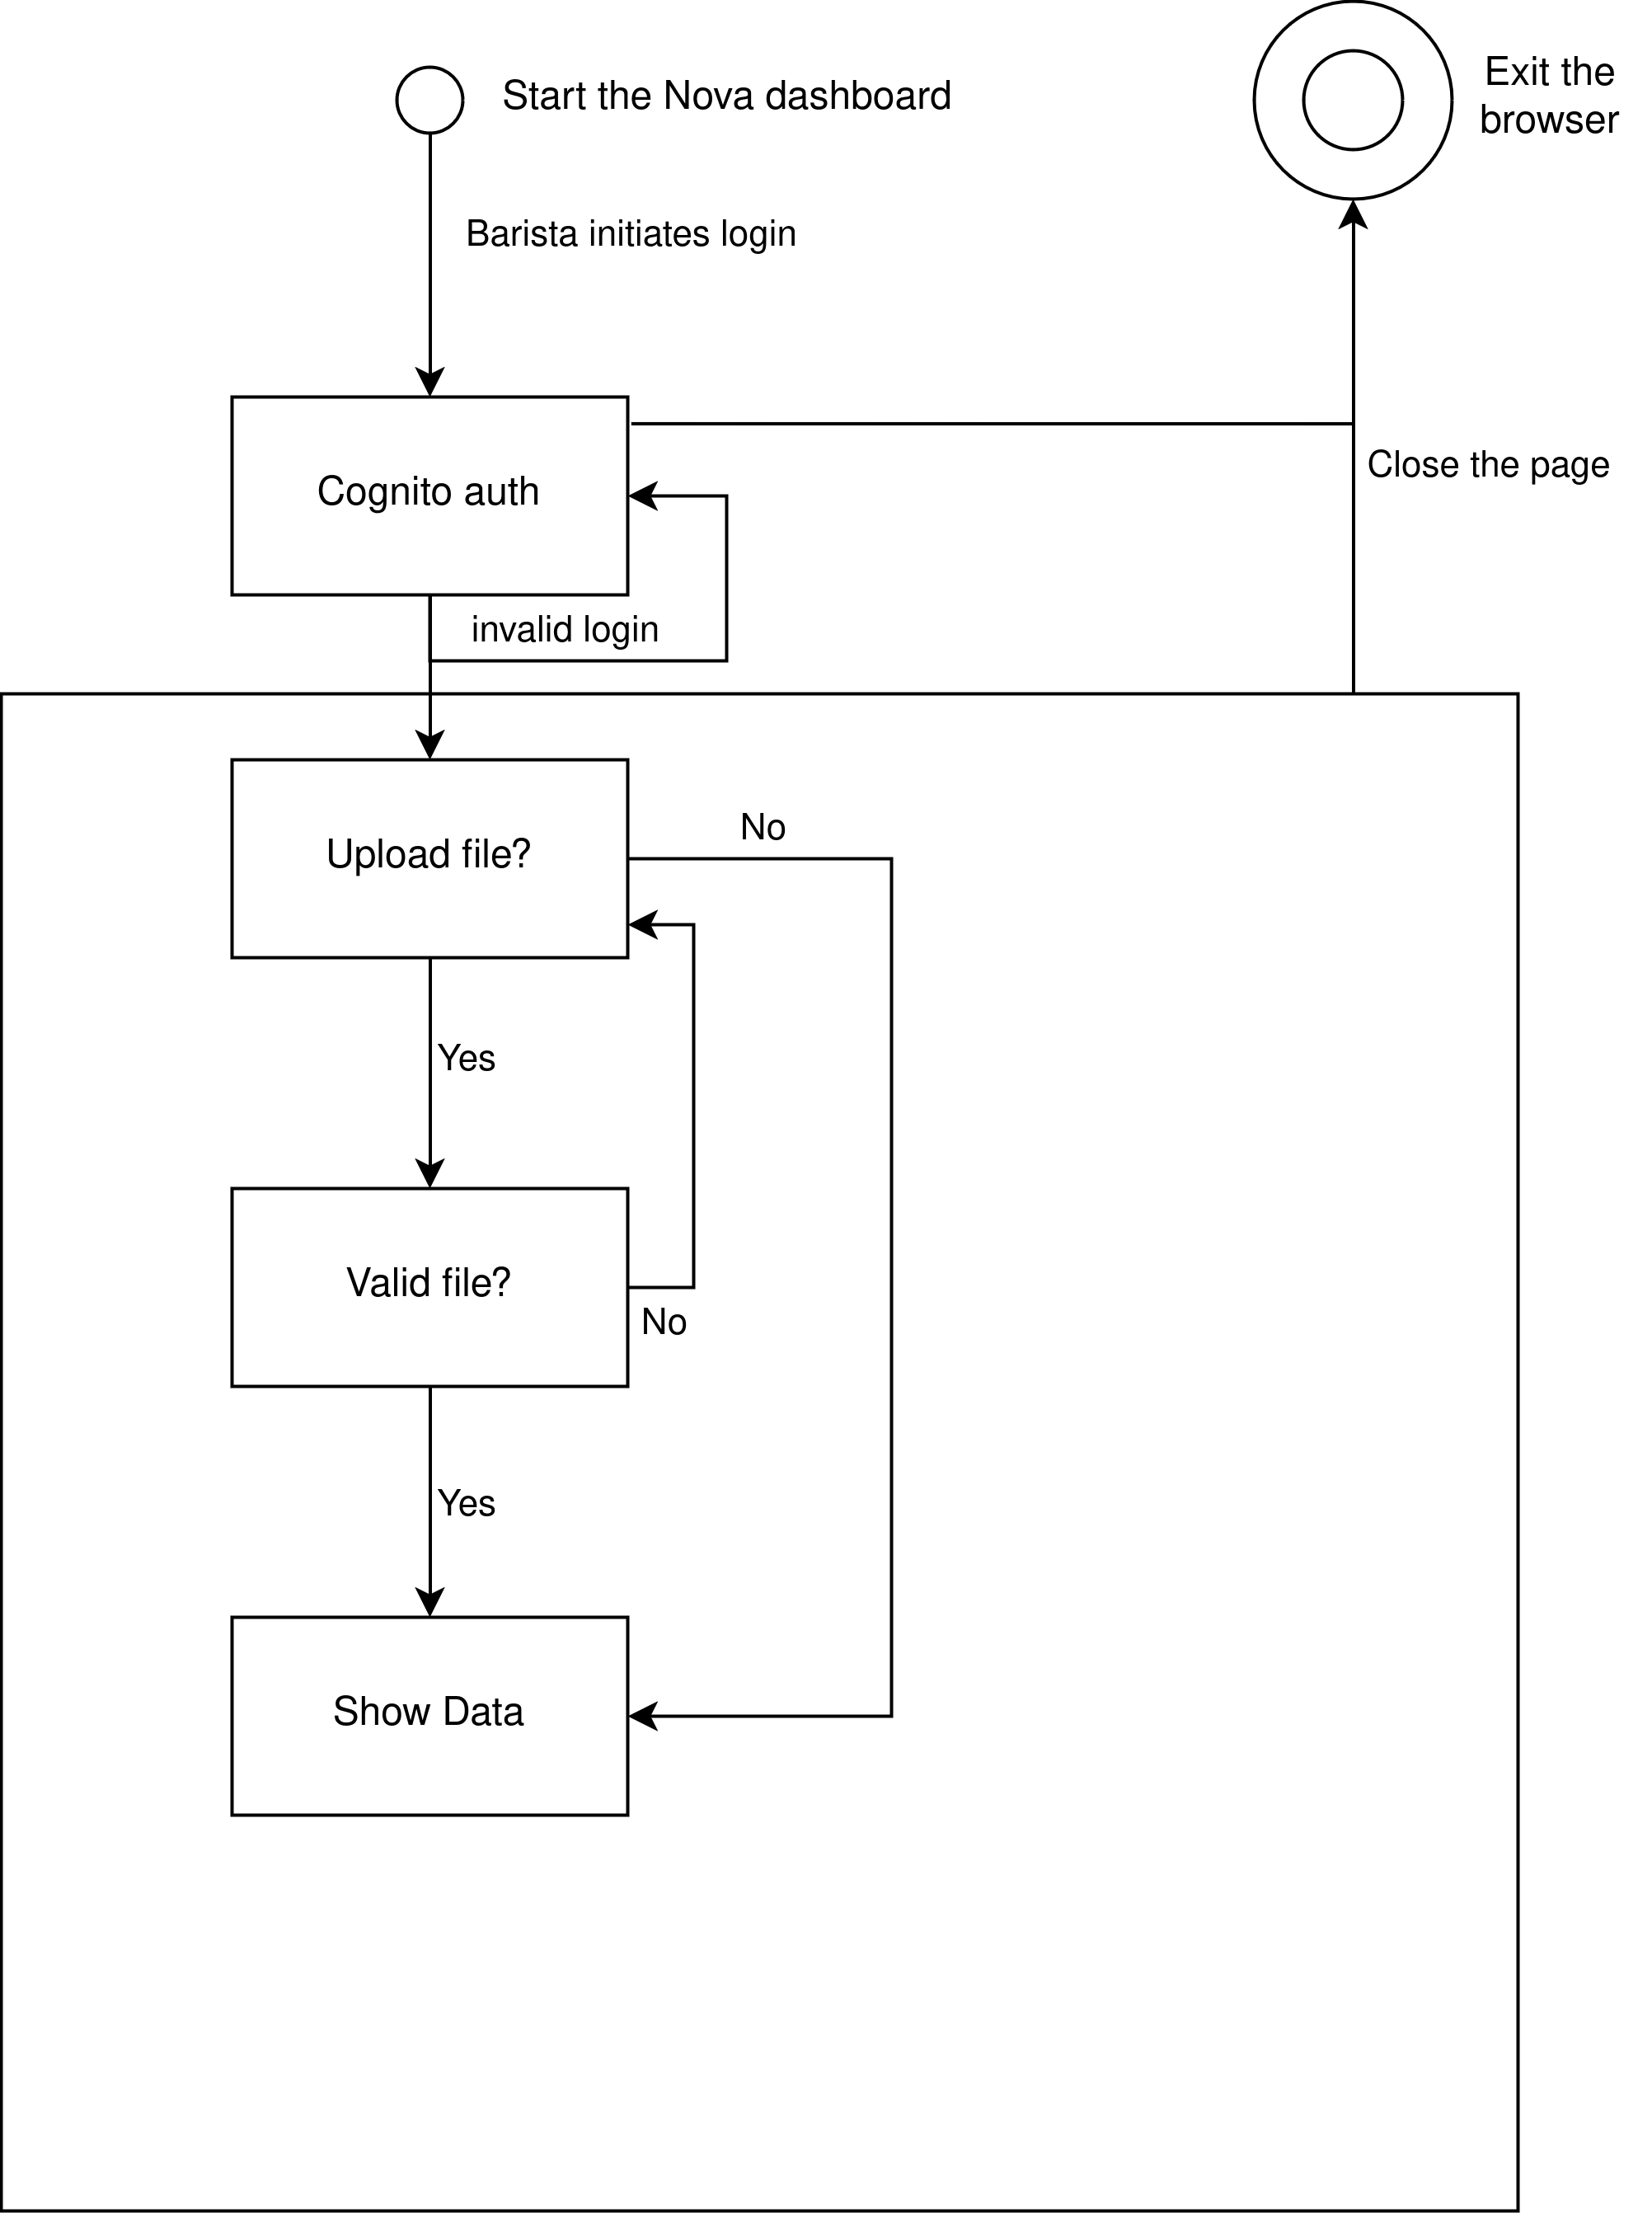
\includegraphics[width=0.7\textwidth]{ada-barista}
    \caption{A diagram showing a barista actors use-case.
    }\label{fig:barista-conditional}
\end{figure}

% textidote: ignore begin
\subsubsection{Diagram viewing}\label{subsubsec:diagram_viewing_usecase}
% textidote: ignore end

After a successful login, the user will immediately be directed to the dashboard that includes all diagrams.
Here the user can customize different aspects of the diagrams to get the easiest overview of their current problem.

% textidote: ignore begin
\subsubsection{Account handling}\label{subsubsec:account_handling_usecase}
% textidote: ignore end

Account handling is only possible for owners, the owners will then send an action to AWS Cognito, which will
do the actual creation, deletion or updating of users.
The use case for account handling can be seen in Figure~\ref{fig:owner-conditional}.

\begin{figure}[H]
    \centering
    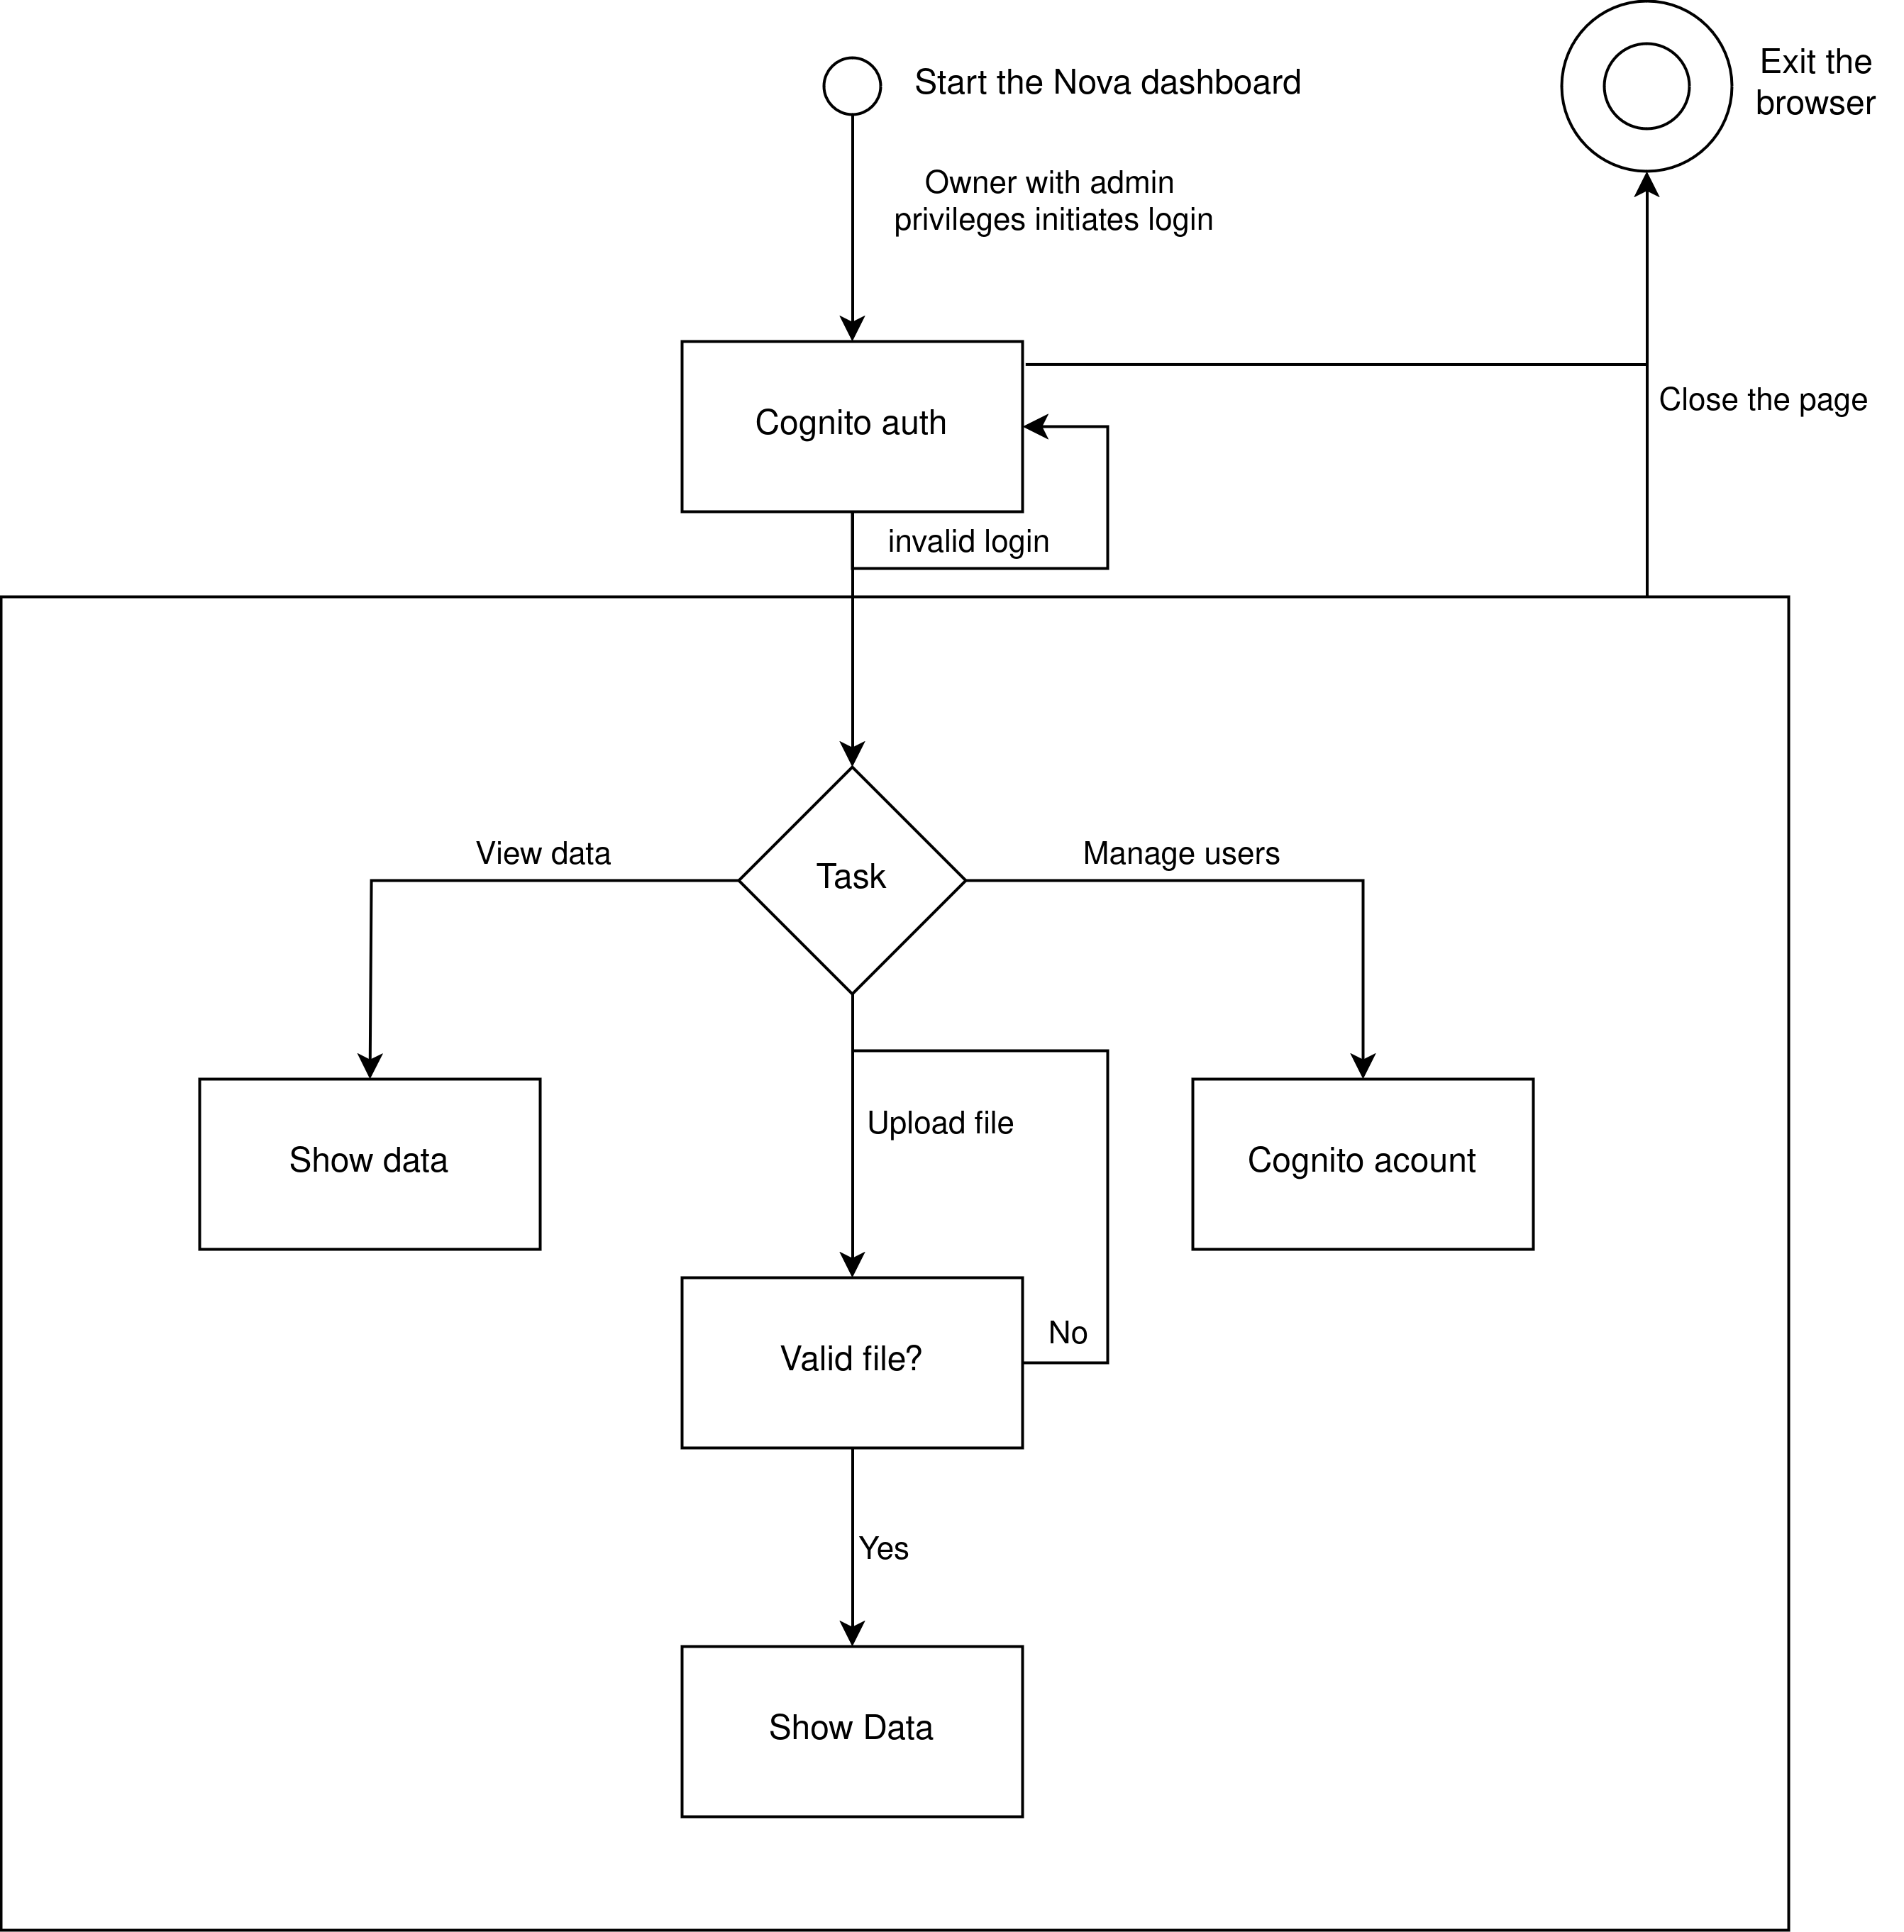
\includegraphics[width=0.9\textwidth]{ada-owner}
    \caption{A diagram showing an owner actors use-case.
    }\label{fig:owner-conditional}
\end{figure}

\subsection{Functions}\label{subsec:functions}

In this section we will analyze the functions of the system.
There are four different function types, hereby Update, Signal, Read and Compute~\cite{mathiassen2018}.
In short, the different function types have the following meanings:

\begin{itemize}
    \item \textbf{Update} functions are initiated by a problem domain event and changes state.
    \item \textbf{Signal} functions are initiated by a change in the state of a model and react accordingly.
    \item \textbf{Read} functions are initiated by an actor and retrieves and displays relevant information about a
    model.
    \item \textbf{Compute} functions are initiated by an actor when there is a need for information processing, data
    transformation or calculation and displays the result.
\end{itemize}

There are also four different complexities, hereby Simple, Medium, Complex and Very complex~\cite{mathiassen2018}.
In short, the different function complexities have the following meanings:

\begin{itemize}
    \item \textbf{Simple} functions perform straightforward operations on a single attribute of an object.
    \item \textbf{Medium} functions create and manipulate single objects.
    \item \textbf{Complex} functions involve interaction between multiple objects.
    They may also have conditional logic.
    \item \textbf{Very complex} functions have several goals and involve several objects and processes.
    They also have branching and multiple decision capabilities among others.
\end{itemize}

In Table~\ref{tab:functions} are all non-trivial functions outlined.
For clarity, we define trivial functions to be basic utility functions and one-line functions, such as getter-functions.
All of these functions are derived from a combination of the use-cases section in Section~\ref{subsec:use-cases},
the section about actors in Section~\ref{subsec:actors}, the event table in Section~\ref{subsec:event-table} and the
section about classes in Section~\ref{subsec:classes-objects-and-structure}.

\begin{table}[h]
    \centering
    \resizebox{\columnwidth}{!}{%
        \begin{tabular}{ccc}
            \toprule
            \textbf{Function name}
            & \textbf{Type}
            & \textbf{Complexity}
            \\ \midrule
            Find user information
            & Read
            & Simple
            \\ \midrule
            Find products by category
            & Read
            & Medium
            \\ \midrule
            Create user session
            & Update
            & Medium
            \\ \midrule
            Validate user session
            & Compute
            & Medium
            \\ \midrule
            Format data
            & Compute
            & Complex
            \\ \midrule
            Validate and process CSV file
            & Compute
            & Very complex
            \\ \bottomrule
        \end{tabular}%
    }
    \caption{Table of all functions and their respective assigned types and complexities.
    Trivial functions are excluded.
    }\label{tab:functions}
\end{table}

The~\textit{Validate and process CSV file} function is classified as very complex due to the number of different
sub-functions it contains.
In Table~\ref{tab:functions-validate-and-process-csv-file} all non-trivial sub-functions regarding
the~\textit{Validate and process CSV file} function are further clarified.

\begin{table}[h]
    \centering
    \resizebox{\columnwidth}{!}{%
        \begin{tabular}{ccc}
            \toprule
            \textbf{Function name}
            & \textbf{Type}
            & \textbf{Complexity}
            \\ \midrule
            Validate CSV file type
            & Read
            & Simple
            \\ \midrule
            Handle exceptions
            & Signal
            & Simple
            \\ \midrule
            Save CSV contents
            & Update
            & Medium
            \\ \midrule
            Create additional meta-attributes
            & Update
            & Medium
            \\ \midrule
            Match CSV field to model
            & Compute
            & Medium
            \\ \midrule
            Check for duplicates
            & Compute
            & Medium
            \\ \bottomrule
        \end{tabular}%
    }
    \caption{Table of all sub-functions and their respective type and complexity regarding the very complex parent
    function~\textit{Validate and process CSV file} seen in Table~\ref{tab:functions}.
    Trivial functions are excluded.
    }\label{tab:functions-validate-and-process-csv-file}
\end{table}

